\clearpage

\section{Results}

In this section we provide the results of the inclusive and targeted searches. 
The observed and predicted \MET\ distributions for the inclusive analysis are indicated in Fig.~\ref{fig:results_incl}. 
A summary of the results in the signal regions is provided in Table~\ref{tab:results_incl}. 
Good agreement is observed between the data and the predicted background over the full \MET\ range.
%The separate results for the ee and $\mu\mu$ channels are presented in App.~\ref{app:results}.

\begin{figure}[!h]
\begin{center}
\begin{tabular}{cc}
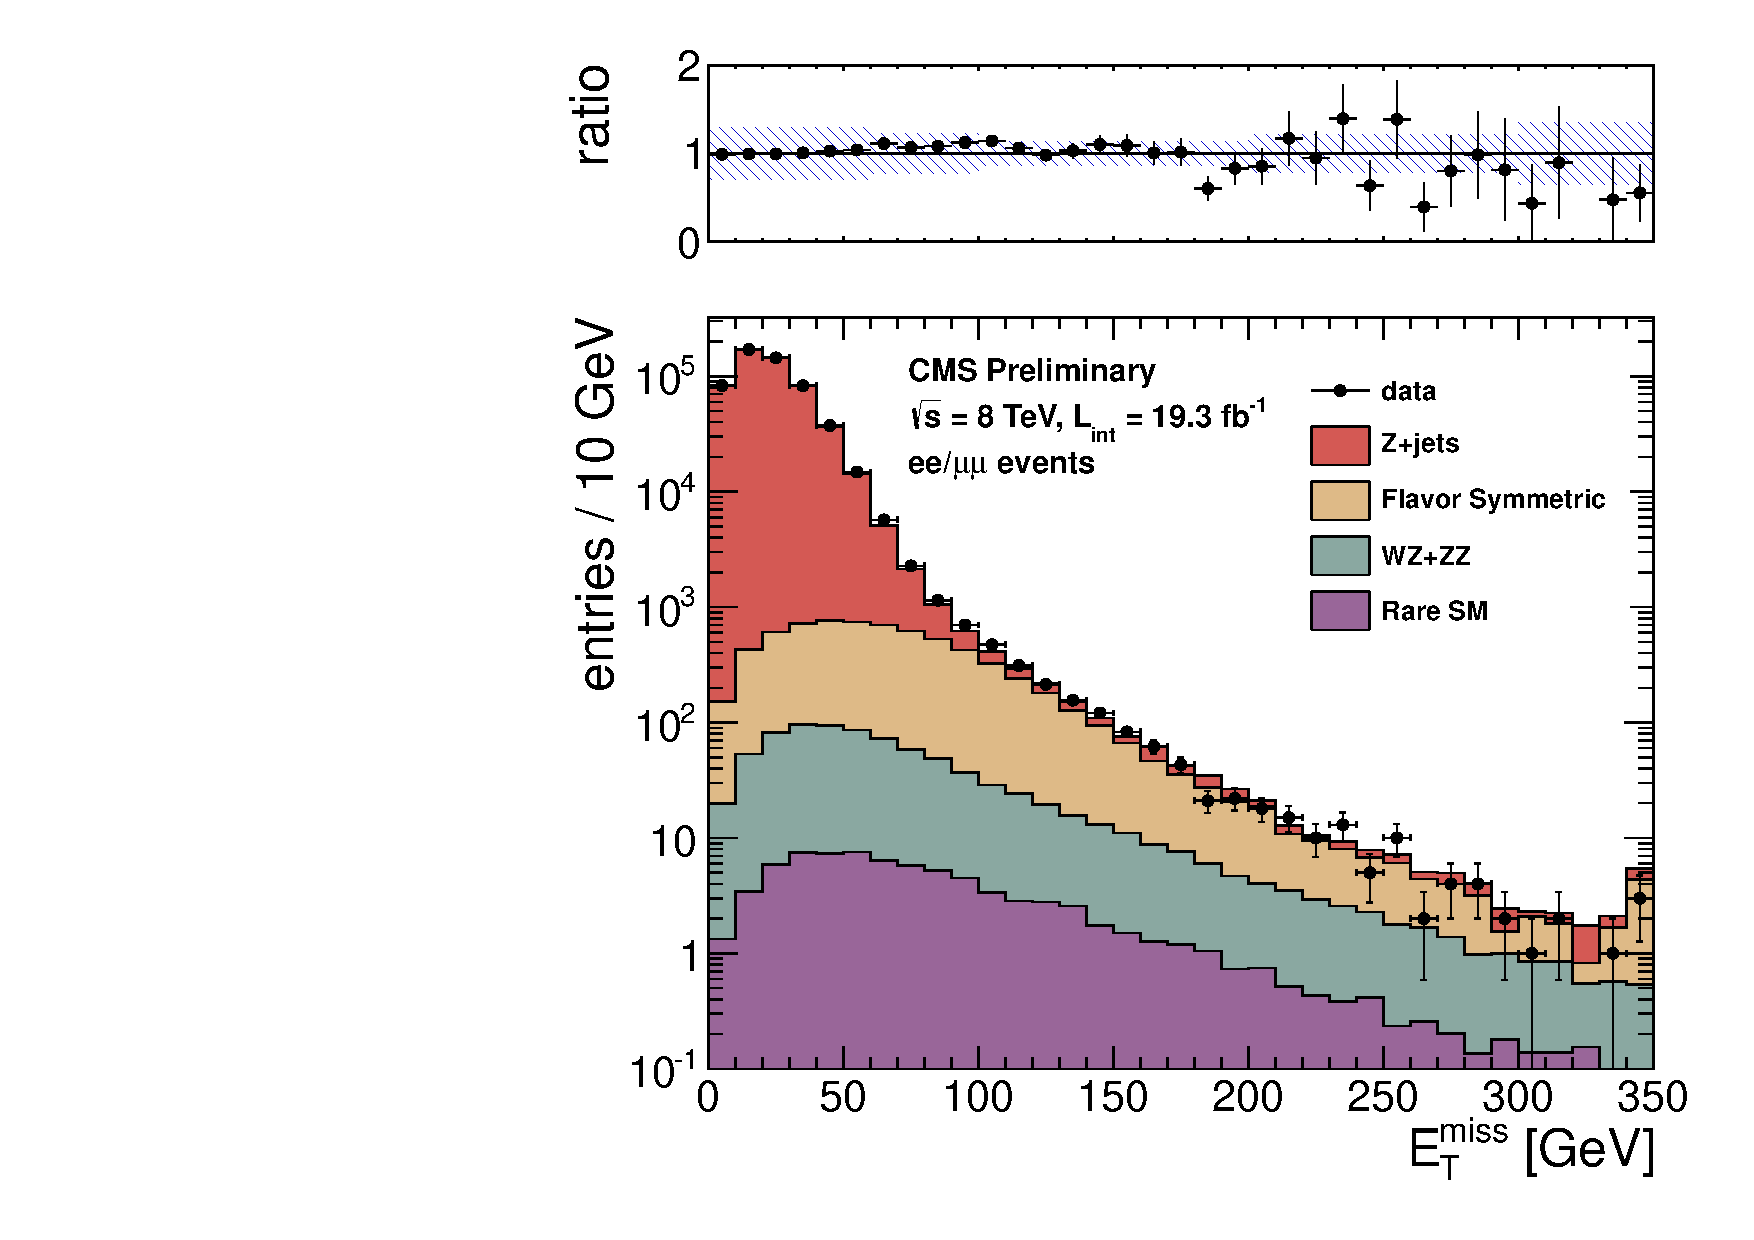
\includegraphics[width=0.6\textwidth]{plots/pfmet_all_19fb.pdf}
\end{tabular}
\caption{Results of the inclusive analysis. The observed \MET\ distribution (black points) is compared with the sum of the predicted \MET\
distributions from \zjets, flavor-symmetric backgrounds, and WZ+ZZ backgrounds. The ratio of observed to predicted yields in each bin is
indicated. The error bars indicate the statistical uncertainty in the data and the shaded band indicates the total background uncertainty.
\label{fig:results_incl}
}
\end{center}
\end{figure}



\begin{table}[htb]
\begin{center}
\footnotesize
\caption{\label{tab:results_incl} Summary of results in the inclusive analysis. The total background is the sum of the \zjets\ background predicted from
the \MET\ templates method (\zjets\ bkg), the flavor-symmetric background predicted from e$\mu$ events (FS bkg), and the WZ and ZZ backgrounds predicted from MC
(WZ bkg and ZZ bkg). All uncertainties include both the statistical and systematic components. The Gaussian significance of the deviation between the data 
and total background is indicated for signal regions with at least 20 observed events. }
\begin{tabular}{l|c|c|c|c|c|c}

\hline
\hline

\begin{comment}
Using pfmet out-of-the-box
WZ/ZZ selection : ((((((leptype==0 && (ee==1 || isdata==0))||(leptype==1 && (mm==1 || isdata==0)))&&(ngennu>0))&&(csc==0 && hbhe==1 && hcallaser==1 && ecaltp==1 && trkfail==1 && eebadsc==1 && hbhenew==1))&&(dilmass>81 && dilmass<101))&&(njets>=2))&&(lep1.pt()>20.0 && lep2.pt()>20.0)
WZ/ZZ weight    : weight * 19.3 * vtxweight * trgeff
Opening ../output/V00-02-00/babylooper_data_53X_2012ALL_PhotonStitchedTemplate_pfmet.root
B-veto?   0
K         0.14
ee+mm channels: scale em yield by 0.98
Yields in 0-60 GeV region
data   : 533201
gjets  : 537544
OF     : 2979.3
WZ     : 348.772
ZZ     : 49.8729
Rare   : 33.0953
Scaling gjets by : 0.985576
SF events 544614
OF events 44581
\end{comment}

                      &   \MET\ 0--30 GeV   &  \MET\ 30--60 GeV   & \MET\ 60--100 GeV   &\MET\ 100--200 GeV   &\MET\ 200--300 GeV   & \MET\ $>$ 300 GeV  \\
\hline
        \zjets\ bkg   &399165 $\pm$ 119750   &130625 $\pm$ 39188   &   6652 $\pm$ 1996   &      266 $\pm$ 80   &    12.1 $\pm$ 3.8   &     3.0 $\pm$ 1.0  \\
             FS bkg   &    1031 $\pm$ 160   &    1948 $\pm$ 302   &    2056 $\pm$ 319   &    1022 $\pm$ 159   &   51.0 $\pm$ 15.1   &     7.4 $\pm$ 4.4  \\
             WZ bkg   &  128.9 $\pm$ 90.2   & 219.9 $\pm$ 153.9   & 158.2 $\pm$ 110.7   &   86.4 $\pm$ 60.5   &    11.8 $\pm$ 8.3   &     3.3 $\pm$ 3.3  \\
             ZZ bkg   &    15.9 $\pm$ 8.0   &   34.0 $\pm$ 17.0   &   36.5 $\pm$ 18.2   &   33.8 $\pm$ 16.9   &     6.8 $\pm$ 3.4   &     2.0 $\pm$ 2.0  \\
        rare SM bkg   &    10.6 $\pm$ 5.3   &   22.4 $\pm$ 11.2   &   21.9 $\pm$ 11.0   &    19.1 $\pm$ 9.6   &     3.5 $\pm$ 1.8   &     1.2 $\pm$ 1.2  \\
\hline
          total bkg   &400351 $\pm$ 119750   &132850 $\pm$ 39190   &   8925 $\pm$ 2025   &    1428 $\pm$ 189   &   85.3 $\pm$ 18.1   &    17.0 $\pm$ 6.1  \\
               data   &            398148   &            135053   &              9816   &              1507   &                83   &                 7  \\
       significance   &      -0.0$\sigma$   &       0.1$\sigma$   &       0.4$\sigma$   &       0.4$\sigma$   &      -0.1$\sigma$   &   \\

\hline
\hline
\end{tabular}
\end{center}
\end{table}

\clearpage

The observed and predicted \MET\ distributions for the targeted analysis are indicated in Fig.~\ref{fig:results_targ}. 
A summary of the results in the signal regions is provided in Table~\ref{tab:results_targ}. 
Good agreement is observed between the data and the predicted background over the full \MET\ range.
%The separate results for the ee and $\mu\mu$ channels are presented in App.~\ref{app:results}.

\begin{figure}[!h]
\begin{center}
\begin{tabular}{cc}
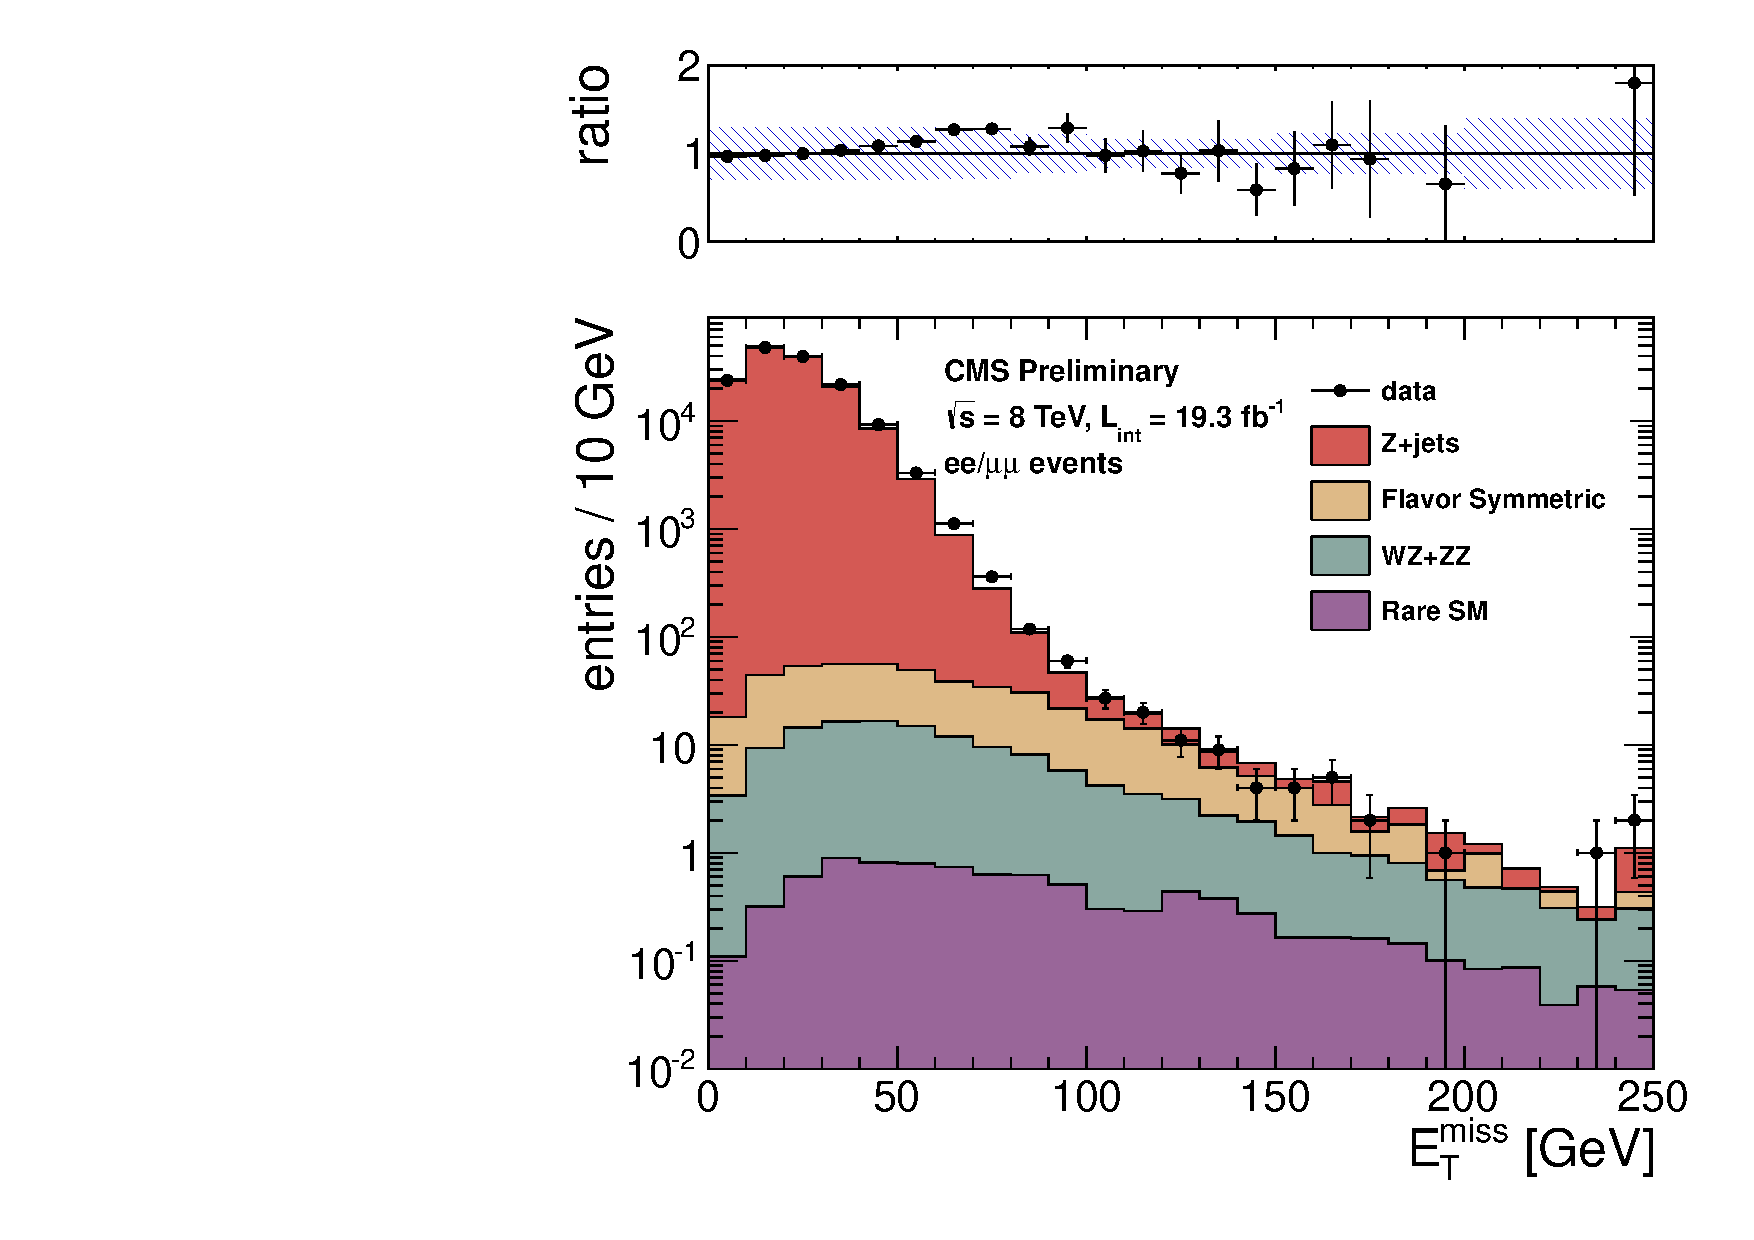
\includegraphics[width=0.5\textwidth]{plots/pfmet_bveto_all_19fb.pdf}
\end{tabular}
\caption{Results of the $\rm{Z}+{dijet}$ analysis. The observed $\rm{E_{T}^{miss}}$ distribution (black points) is compared with the sum of the predicted $\rm{E_{T}^{miss}}$
distributions from $\rm{Z}+\rm{jets}$, flavor-symmetric (FS), sum of WZ and ZZ (WZ+ZZ), and rare SM backgrounds. The ratio of observed to predicted yields in each bin is
indicated. The error bars indicate the statistical uncertainty in the data and the shaded band indicates the total background uncertainty.
\label{fig:results_targ}
}
\end{center}
\end{figure}



\begin{table}[htb]
\begin{center}
\footnotesize
\caption{\label{tab:results_targ}\footnotesize Summary of results in the targeted analysis. The total background is the sum of the \zjets\ background predicted from
the \MET\ templates method (\zjets\ bkg), the flavor-symmetric background predicted from e$\mu$ events (FS bkg), and the WZ and ZZ backgrounds predicted from MC
(WZ bkg and ZZ bkg). All uncertainties include both the statistical and systematic components. The Gaussian significance of the deviation between the data 
and total background is indicated for signal regions with at least 20 observed events. }
\begin{tabular}{l|c|c|c|c}


%Using pfmet out-of-the-box
%Apply mjj cut in templates
%WZ/ZZ selection : ((((((((leptype==0 && (ee==1 || isdata==0))||(leptype==1 && (mm==1 || isdata==0)))&&(ngennu>0))&&(csc==0 && hbhe==1 && hcallaser==1 && ecaltp==1 && trkfail==1 && eebadsc==1 && hbhenew==1))&&(dilmass>81 && dilmass<101))&&(njets>=2))&&(lep1.pt()>20.0 && lep2.pt()>20.0))&&(nlep==2))&&(mjj>70.0 && mjj<110.0)
%WZ/ZZ weight    : weight * 19.3 * vtxweight * trgeff
%Opening ../output/V00-02-00/babylooper_data_53X_2012ALL_PhotonStitchedTemplate_pfmet_bveto_mjjcut.root
%B-veto?   1
%K         0.13
%ee+mm channels: scale em yield by 0.98
%Yields in 0-60 GeV region
%data   : 145069
%gjets  : 145529
%OF     : 201.547
%WZ     : 57.8524
%ZZ     : 13.8061
%Rare   : 3.53803
%Scaling gjets by : 0.994937
%SF events 146811
%OF events 2632

\hline
\hline
                      &   \MET\ 0--30 GeV   &  \MET\ 30--60 GeV   &  \MET\ 60--80 GeV   & \MET\ 80--100 GeV   \\
\hline
        \zjets\ bkg   &111698 $\pm$ 33511   &  33094 $\pm$ 9929   &    1141 $\pm$ 343   &      106 $\pm$ 33   \\
             FS bkg   &   88.8 $\pm$ 15.0   &      113 $\pm$ 19   &    51.5 $\pm$ 8.9   &    38.0 $\pm$ 6.6   \\
             WZ bkg   &   21.5 $\pm$ 15.0   &   36.4 $\pm$ 25.5   &   15.2 $\pm$ 10.6   &     8.7 $\pm$ 6.1   \\
             ZZ bkg   &     4.6 $\pm$ 2.3   &     9.2 $\pm$ 4.6   &     4.9 $\pm$ 2.5   &     4.1 $\pm$ 2.1   \\
        rare SM bkg   &     1.0 $\pm$ 0.5   &     2.5 $\pm$ 1.3   &     1.4 $\pm$ 0.7   &     1.1 $\pm$ 0.6   \\
\hline
          total bkg   &111814 $\pm$ 33511   &  33255 $\pm$ 9929   &    1214 $\pm$ 344   &      158 $\pm$ 34   \\
               data   &            110883   &             34186   &              1478   &               178   \\
       significance   &      -0.0$\sigma$   &       0.1$\sigma$   &       0.8$\sigma$   &       0.6$\sigma$   \\
\hline
\hline

                      &\MET\ 100--120 GeV   &\MET\ 120--150 GeV   &\MET\ 150--200 GeV   & \MET\ $>$ 200 GeV  \\
\hline
        \zjets\ bkg   &    10.8 $\pm$ 3.4   &     6.2 $\pm$ 2.1   &     4.5 $\pm$ 2.6   &     0.5 $\pm$ 0.2  \\
             FS bkg   &    23.4 $\pm$ 4.2   &    14.0 $\pm$ 2.7   &     6.1 $\pm$ 2.5   &     0.8 $\pm$ 0.4  \\
             WZ bkg   &     4.7 $\pm$ 3.3   &     3.7 $\pm$ 2.6   &     2.2 $\pm$ 1.6   &     1.0 $\pm$ 1.0  \\
             ZZ bkg   &     2.4 $\pm$ 1.2   &     2.6 $\pm$ 1.3   &     1.8 $\pm$ 0.9   &     1.6 $\pm$ 1.6  \\
        rare SM bkg   &     0.6 $\pm$ 0.3   &     1.1 $\pm$ 0.6   &     0.7 $\pm$ 0.4   &     0.5 $\pm$ 0.5  \\
\hline
          total bkg   &    41.9 $\pm$ 6.5   &    27.5 $\pm$ 4.5   &    15.4 $\pm$ 4.1   &     4.3 $\pm$ 2.0  \\
               data   &                47   &                24   &                12   &                 3  \\
       significance   &       0.5$\sigma$   &      -0.5$\sigma$   &                     &                    \\
\hline
\hline

\end{tabular}
\end{center}
\end{table}

\clearpage
